\documentclass[tikz,12pt,border=2pt]{standalone}
\usepackage[T1]{fontenc}
\usetikzlibrary{arrows.meta,positioning,calc}
\definecolor{accent}{RGB}{31,84,140}
\definecolor{accentlight}{RGB}{200,214,232}
\begin{document}
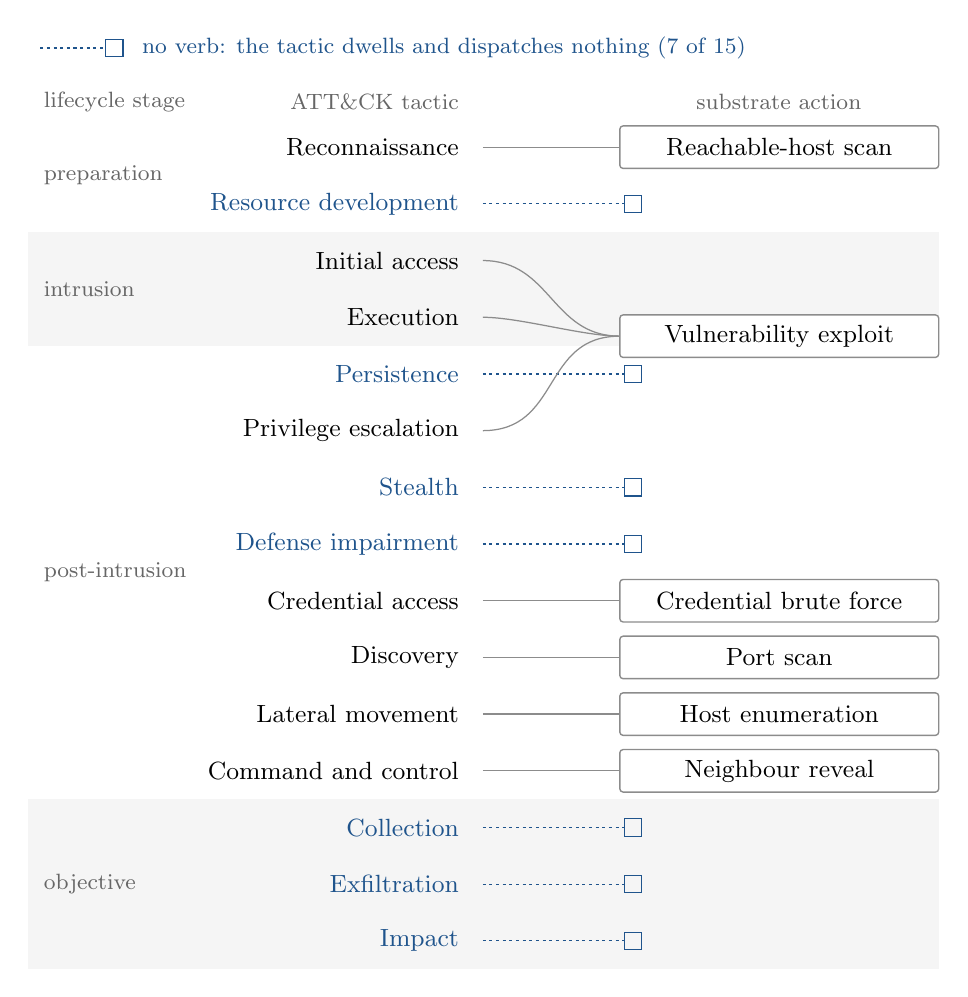
\begin{tikzpicture}[x=1cm,y=1cm,>={Stealth[length=1.6mm]},every node/.style={font=\small}]
\node[anchor=west,font=\footnotesize,text=black!60] at (0.08,-0.360) {preparation};
\fill[black!4] (0.00,-1.08) rectangle (11.57,-2.52);
\node[anchor=west,font=\footnotesize,text=black!60] at (0.08,-1.800) {intrusion};
\node[anchor=west,font=\footnotesize,text=black!60] at (0.08,-5.400) {post-intrusion};
\fill[black!4] (0.00,-8.28) rectangle (11.57,-10.44);
\node[anchor=west,font=\footnotesize,text=black!60] at (0.08,-9.360) {objective};
\draw[accent,line width=0.4pt,dash pattern=on 1.1pt off 1.3pt] (0.16,1.260) -- (0.99,1.260);
\draw[accent,line width=0.4pt] (0.99,1.150) rectangle (1.21,1.370);
\node[anchor=west,font=\footnotesize,text=accent] at (1.33,1.260) {no verb: the tactic dwells and dispatches nothing (7 of 15)};
\node[anchor=west,font=\footnotesize,text=black!60] at (0.08,0.58) {lifecycle stage};
\node[anchor=east,font=\footnotesize,text=black!60] at (5.60,0.58) {ATT\&CK tactic};
\node[anchor=center,font=\footnotesize,text=black!60] at (9.54,0.58) {substrate action};
\node[anchor=east,text=black] at (5.60,0.000) {Reconnaissance};
\node[anchor=east,text=accent] at (5.60,-0.720) {Resource development};
\node[anchor=east,text=black] at (5.60,-1.440) {Initial access};
\node[anchor=east,text=black] at (5.60,-2.160) {Execution};
\node[anchor=east,text=accent] at (5.60,-2.880) {Persistence};
\node[anchor=east,text=black] at (5.60,-3.600) {Privilege escalation};
\node[anchor=east,text=accent] at (5.60,-4.320) {Stealth};
\node[anchor=east,text=accent] at (5.60,-5.040) {Defense impairment};
\node[anchor=east,text=black] at (5.60,-5.760) {Credential access};
\node[anchor=east,text=black] at (5.60,-6.480) {Discovery};
\node[anchor=east,text=black] at (5.60,-7.200) {Lateral movement};
\node[anchor=east,text=black] at (5.60,-7.920) {Command and control};
\node[anchor=east,text=accent] at (5.60,-8.640) {Collection};
\node[anchor=east,text=accent] at (5.60,-9.360) {Exfiltration};
\node[anchor=east,text=accent] at (5.60,-10.080) {Impact};
\draw[black!45,line width=0.45pt] (5.78,0.000) .. controls +(0.34,0) and +(-0.34,0) .. (7.52,0.000);
\draw[accent,line width=0.4pt,dash pattern=on 1.1pt off 1.3pt] (5.78,-0.720) -- (7.58,-0.720);
\draw[accent,line width=0.4pt] (7.58,-0.830) rectangle (7.80,-0.610);
\draw[black!45,line width=0.45pt] (5.78,-1.440) .. controls +(0.87,0) and +(-0.87,0) .. (7.52,-2.400);
\draw[black!45,line width=0.45pt] (5.78,-2.160) .. controls +(0.47,0) and +(-0.47,0) .. (7.52,-2.400);
\draw[accent,line width=0.4pt,dash pattern=on 1.1pt off 1.3pt] (5.78,-2.880) -- (7.58,-2.880);
\draw[accent,line width=0.4pt] (7.58,-2.990) rectangle (7.80,-2.770);
\draw[black!45,line width=0.45pt] (5.78,-3.600) .. controls +(1.00,0) and +(-1.00,0) .. (7.52,-2.400);
\draw[accent,line width=0.4pt,dash pattern=on 1.1pt off 1.3pt] (5.78,-4.320) -- (7.58,-4.320);
\draw[accent,line width=0.4pt] (7.58,-4.430) rectangle (7.80,-4.210);
\draw[accent,line width=0.4pt,dash pattern=on 1.1pt off 1.3pt] (5.78,-5.040) -- (7.58,-5.040);
\draw[accent,line width=0.4pt] (7.58,-5.150) rectangle (7.80,-4.930);
\draw[black!45,line width=0.45pt] (5.78,-5.760) .. controls +(0.34,0) and +(-0.34,0) .. (7.52,-5.760);
\draw[black!45,line width=0.45pt] (5.78,-6.480) .. controls +(0.34,0) and +(-0.34,0) .. (7.52,-6.480);
\draw[black!45,line width=0.45pt] (5.78,-7.200) .. controls +(0.34,0) and +(-0.34,0) .. (7.52,-7.200);
\draw[black!45,line width=0.45pt] (5.78,-7.920) .. controls +(0.34,0) and +(-0.34,0) .. (7.52,-7.920);
\draw[accent,line width=0.4pt,dash pattern=on 1.1pt off 1.3pt] (5.78,-8.640) -- (7.58,-8.640);
\draw[accent,line width=0.4pt] (7.58,-8.750) rectangle (7.80,-8.530);
\draw[accent,line width=0.4pt,dash pattern=on 1.1pt off 1.3pt] (5.78,-9.360) -- (7.58,-9.360);
\draw[accent,line width=0.4pt] (7.58,-9.470) rectangle (7.80,-9.250);
\draw[accent,line width=0.4pt,dash pattern=on 1.1pt off 1.3pt] (5.78,-10.080) -- (7.58,-10.080);
\draw[accent,line width=0.4pt] (7.58,-10.190) rectangle (7.80,-9.970);
\draw[black!45,line width=0.5pt,fill=white,rounded corners=1.2pt] (7.52,-0.270) rectangle (11.57,0.270);
\node[anchor=center] at (9.545,0.000) {Reachable-host scan};
\draw[black!45,line width=0.5pt,fill=white,rounded corners=1.2pt] (7.52,-2.670) rectangle (11.57,-2.130);
\node[anchor=center] at (9.545,-2.400) {Vulnerability exploit};
\draw[black!45,line width=0.5pt,fill=white,rounded corners=1.2pt] (7.52,-6.030) rectangle (11.57,-5.490);
\node[anchor=center] at (9.545,-5.760) {Credential brute force};
\draw[black!45,line width=0.5pt,fill=white,rounded corners=1.2pt] (7.52,-6.750) rectangle (11.57,-6.210);
\node[anchor=center] at (9.545,-6.480) {Port scan};
\draw[black!45,line width=0.5pt,fill=white,rounded corners=1.2pt] (7.52,-7.470) rectangle (11.57,-6.930);
\node[anchor=center] at (9.545,-7.200) {Host enumeration};
\draw[black!45,line width=0.5pt,fill=white,rounded corners=1.2pt] (7.52,-8.190) rectangle (11.57,-7.650);
\node[anchor=center] at (9.545,-7.920) {Neighbour reveal};
\end{tikzpicture}
\end{document}
